% Chapter Template

\chapter{Experimental Results on Routing Strategies} % Main chapter title

\label{expereince}

\lhead{Chapter 2. \emph{Experimental Results on Routing Strategies}}

\section{Experiment Test Setup}
We tested our experiments on cisco's server with linux containers with different configuration set ups on Lurch. In the case of needs, dynamic modifications also have been added on Lurch to be more interactive for different test scenarios.

In this chapter we will show, test and validate our 4 routing strategies on 2 different setup networks with 5 nodes (medium size) and another one with 17 nodes (large size) each one with customized capacity. We plot rates in Kbps vs time for each link involved in strategy. $\{ai\}$, $i=$1:8 are Access Points and nodes with \textit{NodeID} are Autonomous nodes in the network.
   
In all scenarios we plot the figures of each link by nodeID of connected ends. \textit{In}, \textit{Out} means the direction of packets that come to node. So \textit{In} always is Data packets and Out are Interest packets. As it's clear they are larger than We consider number of hops as cost of link as it is meaningful in ICN architecture.
\textit{TreeOnConsumer}, \textit{TreeOnProducer}, \textit{MinCostMultipath}, \textit{MaxFlow} are 4 different parameters of RoutingNDN module to choose which are done for \textit{Medium} and \textit{Large} size. We have put the result of each case inside the subsection.

In all cases Clients are searching /n/a/noseg chunk and repositories are containing /n folder which has alphabetical letters to like a,b,c,d, ... then chunks of \textit{BigBuckBunny.mp4} are appended to them. Engine of repository is an application called \textit{repo-ng}. 

\section{Strategies on Medium Size NDN Network}


\subsection{TreeOnConsumer}
As figure \ref{TreeOnConsumer} shows, 'luca' and 'jordan' nodes are clients searching '/n/a/noseg' chunk and 'shahab' node is producer of content. The first prefix of content is /n folder.

Figure \ref{treeonconsumer} shows 4 traced rates in which yellow and green one are data packets. Same packets are routed through \textit{TreeOnConsumer} tree to the clients with different rates. In this figure you can see the delay between 'shahab-jordan/In' and 'shahab-luca/In' which is because of capacity difference of between containers. So you have 2 threads on 2 different machines occurring and recorded at the same time.

\begin{figure}[H]

\begin{center}

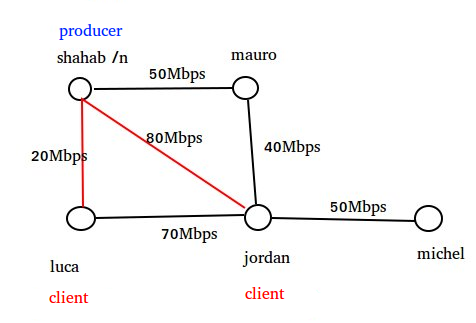
\includegraphics[scale = 0.4]{Figures/TreeOnConsumer.png}

\caption{TreeOnConsumer Tree Medium} \label{TreeOnConsumer} 


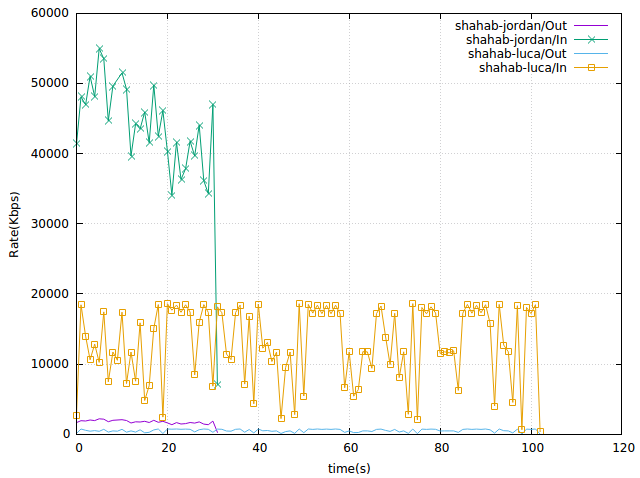
\includegraphics[scale = 0.4]{Figures/treeonconsumer.png}

\caption{TreeOnConsumer (Rate vs Time) Medium} \label{treeonconsumer} 


\end{center}

\end{figure}


\subsection{TreeOnProducer}
Figure \ref{TreeOnProducer} shows 'jordan', a client who searches '/n/a/noseg' and 2 producers ('shahab','mauro') who send packets to client by this strategy using tree of \textit{TreeOnProducer}. 
Figure \ref{treeonproducer} shows as well this downloading traced during time which can be used whenever client wants a high quality content.

Imagine a case in which the clients are searching a very huge amount of data, specially let's say 10 clients that they want to watch a video at the same time through connected base station.

This strategy can be very useful in the case that by understanding multihoming of the core system or backhaul to which base stations are connected.

\begin{figure}[H]

\begin{center}

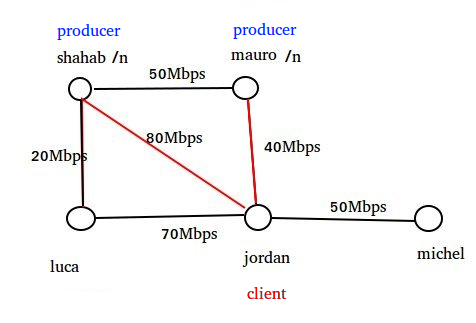
\includegraphics[scale = 0.4]{Figures/TreeOnProducer.png}

\caption{TreeOnProducer Tree Medium} \label{TreeOnProducer} 


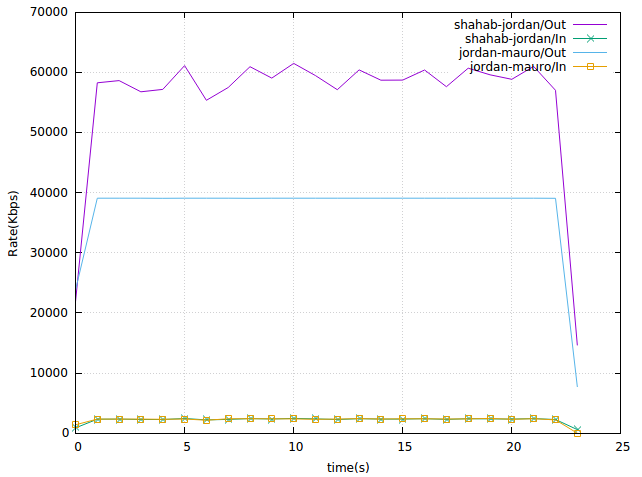
\includegraphics[scale = 0.4]{Figures/treeonproducer.png}

\caption{TreeOnProducer (Rate vs Time) Medium} \label{treeonproducer} 


\end{center}

\end{figure}

\subsection{MinCostMultipath}
Figure \ref{MinCostMultipath} shows \textit{MinCostMultipath} tree of minimum network in which we use number of hops as cost of links. This is the case in which we want to broadcast video livestreaming as we discussed. Same chunk of data are searching at the same time for a live movie like a football match content to all clients.


This figure will be useful when you have a multihoming system in which you are able to download your content from different nodes. This strategy will be a good idea in the case that you have a lot clients on one base station are attached.

This is a co-algorithm of TreeOnConsumer or a way of rethinking of that. In TreeOnConsumer you assume that multi nodes are searching the same content while in TreeOnProducer you have just one client that searches content but with using multihoming advantage of network. 

Whenever the algorithm has created multiple faces for this particular node, the strategy can not no more be \textit{best-route} because this strategy sends just on one face. So in this case we should use another strategy like \textit{multicast}, \textit{load-balance} or \textit{broadcast} to be able to do routing updates and properly sending the packets.
 
Figure \ref{mincost} shows traced data as well.
\begin{figure}[H]

\begin{center}

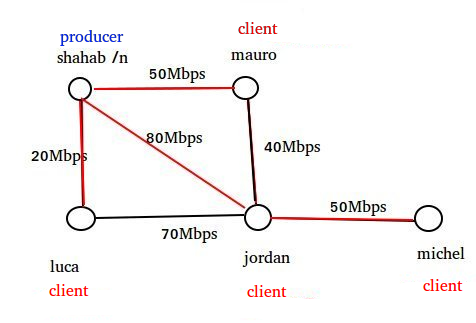
\includegraphics[scale = 0.4]{Figures/MinCostMultipath.png}

\caption{MinCostMultipath Tree Medium} \label{MinCostMultipath} 

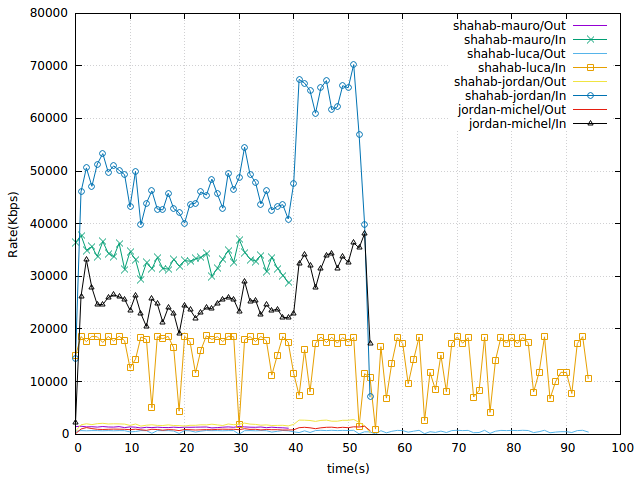
\includegraphics[scale = 0.4]{Figures/mincostmultipath.png}
\caption{MinCostMultipath (Rate vs Time) Medium} \label{mincost} 

\end{center}

\end{figure}

\subsection{MaxFlow}
In figure \ref{MaxFlow} 'jordan' node gets information from all of path possible to maximize data throughput.

Figure \ref{maxflow} shows data rates which are maximum for each link. It can be used whenever clients need higher quality data.

You can see for marginal paths you have on the stable rates.
\begin{figure}[H]

\begin{center}

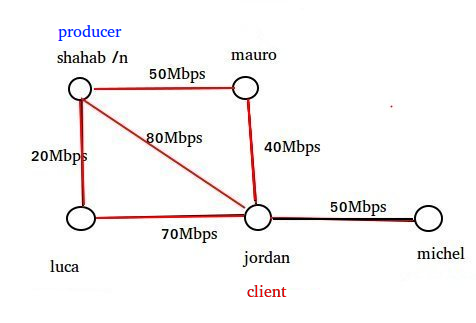
\includegraphics[scale = 0.4]{Figures/MaxFlow.png}

\caption{MaxFlow Medium} \label{MaxFlow} 


\end{center}

\end{figure}

\begin{figure}[H]

\begin{center}

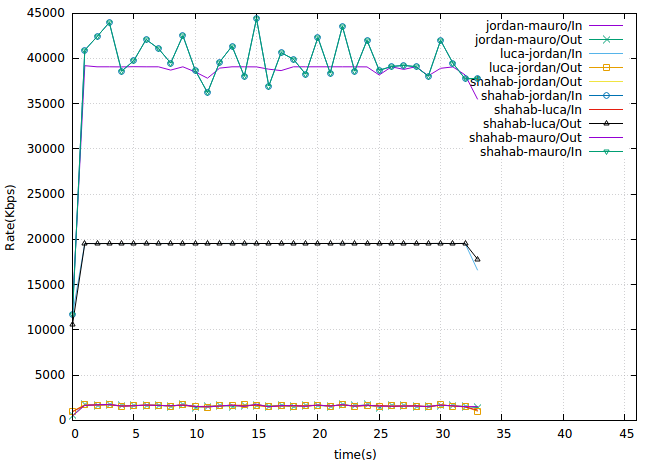
\includegraphics[scale = 0.4]{Figures/maxflow.png}

\caption{MaxFlow (Rate vs Time(s)) Medium} \label{maxflow} 


\end{center}

\end{figure}




 

\section{Strategies on Large Size NDN Networks}

\subsection{TreeOnConsumer}
Figure \ref{TreeOnConsumer_big} shows a red subgraph, $a1, a2, a3, a4$ are Acces Points on which the mobile clients are connected through \textit{TreeOnConsumer} tree on the network.\\
In \ref{treeonconsumer_big}  rates are traced against time as well.

\begin{figure}[H]

\begin{center}

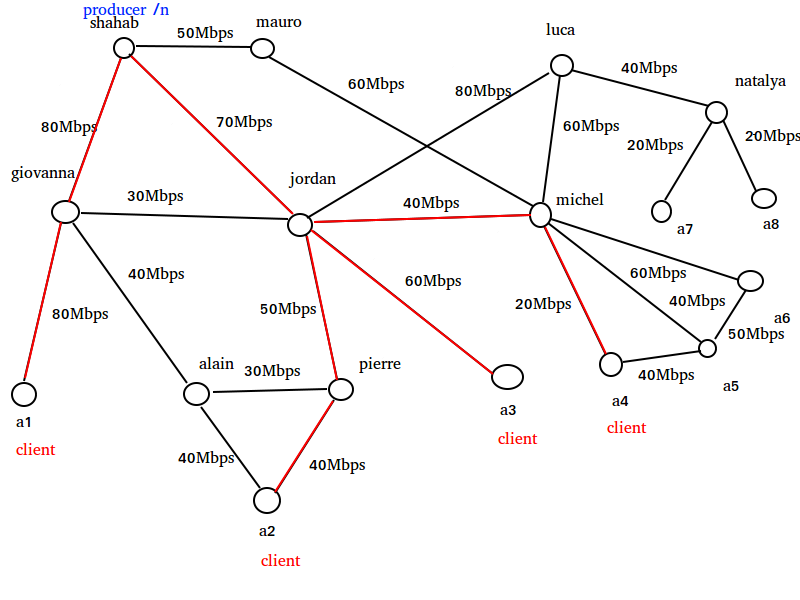
\includegraphics[scale = 0.4]{Figures/TreeOnConsumer_big.png}

\caption{TreeOnConsumer Tree Large} \label{TreeOnConsumer_big} 


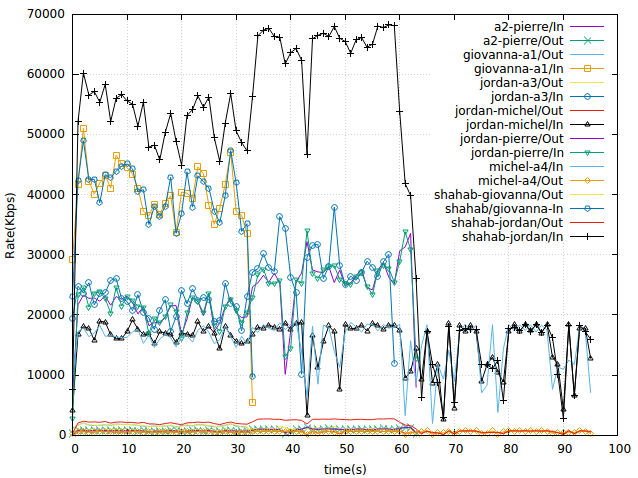
\includegraphics[scale = 0.4]{Figures/treeonconsumer_big.png}

\caption{TreeOnConsumer (Rate vs Time) Large} \label{treeonconsumer_big} 


\end{center}

\end{figure}


Figure \ref{Mob1} shows the first step of client mobility in which the mobile station is attached to node $n10$. Figure \ref{mob1} shows also the Interest/Data packets which are going through shortest paths.

You can see in figure \ref{Mob2} that as soon as mobile client is attached to $n11$ routing update is happened and new routing is traced.

Same case for \ref{Mob3} which is for showing that update can occurred. This update can be designed periodically or to have an algorithm. After we need to know more practical constraints like how much time takes that an routing update happens? The answer depends on what we use for engine forwarder and its implementations. 



\begin{figure}[H]

\begin{center}

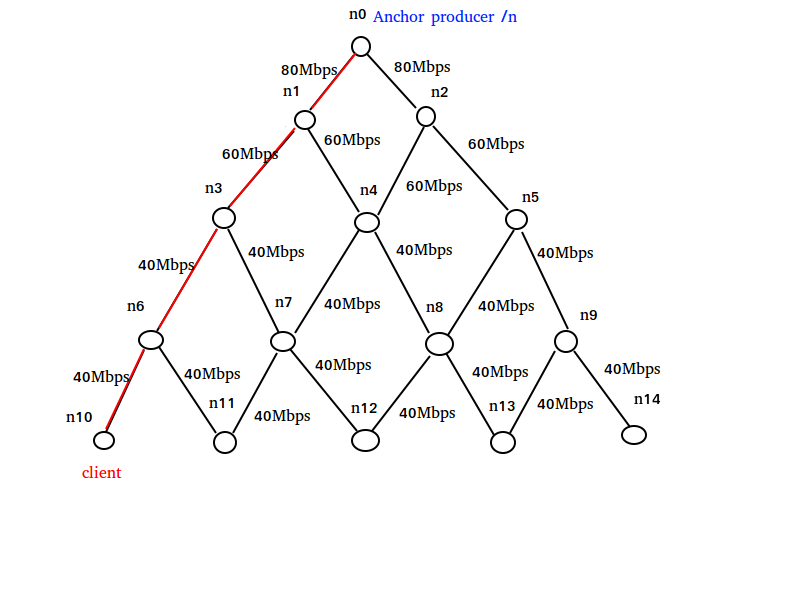
\includegraphics[scale = 0.5]{Figures/Mob1.png}

\caption{TreeOnConsumer Mobility Large} \label{Mob1} 


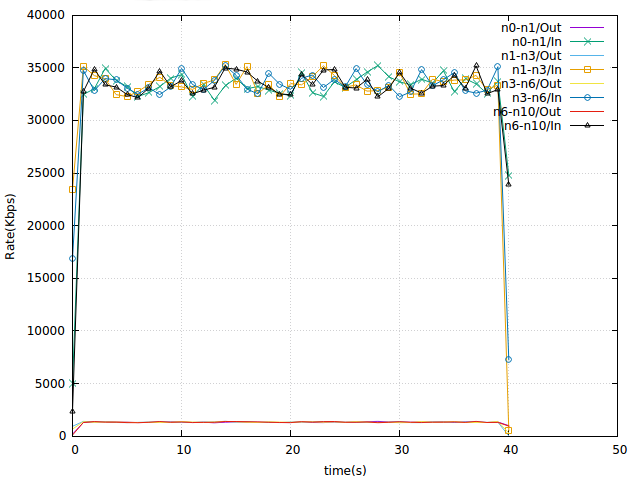
\includegraphics[scale = 0.4]{Figures/mob1.png}

\caption{TreeOnConsumer Mobility (Rate vs Time) Large} \label{mob1} 


\end{center}

\end{figure}

Now in figure \ref{mob1} and \ref{mob2} you see the rates which are changed whenever producer is changed. This changed is done manually in this case.



\begin{figure}[H]

\begin{center}

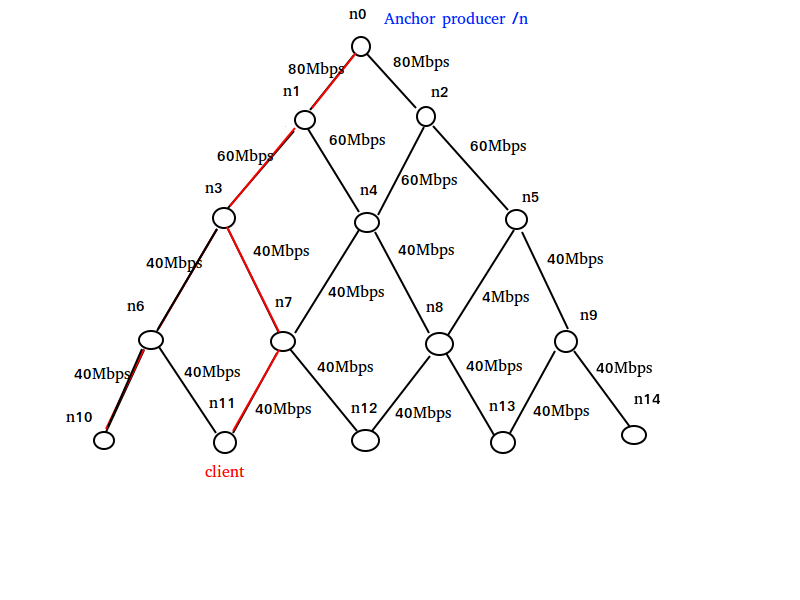
\includegraphics[scale = 0.5]{Figures/Mob2.png}

\caption{TreeOnConsumer Mobility Large} \label{Mob2} 


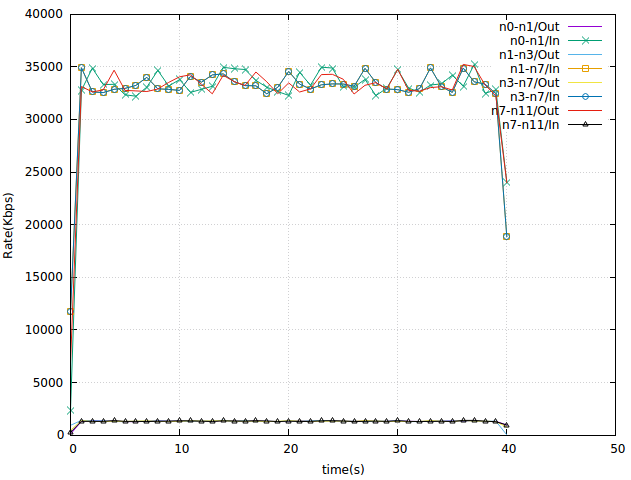
\includegraphics[scale = 0.4]{Figures/mob2.png}

\caption{TreeOnConsumer Mobility (Rate vs Time) Large} \label{mob2} 


\end{center}

\end{figure}

\begin{figure}[H]

\begin{center}

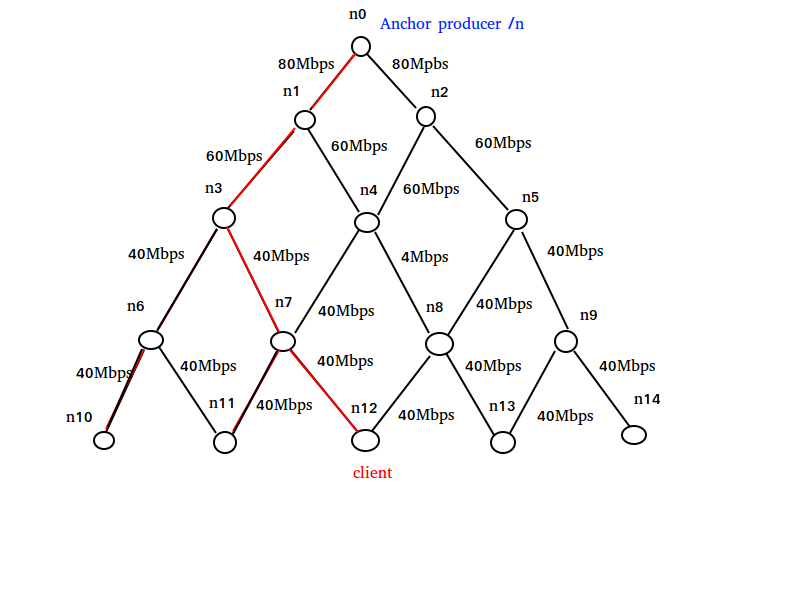
\includegraphics[scale = 0.5]{Figures/Mob3.png}

\caption{TreeOnConsumer Mobility Large} \label{Mob3} 


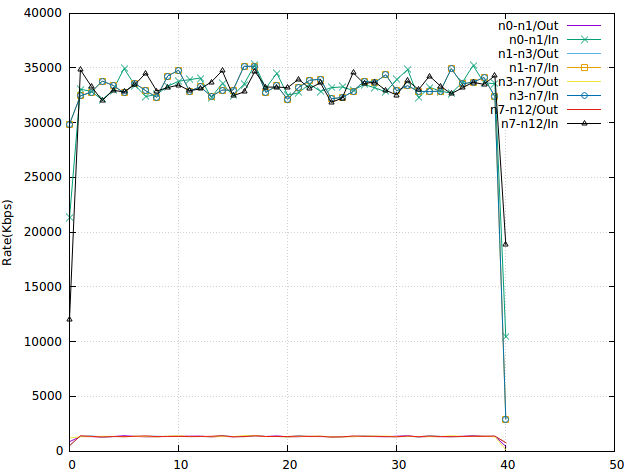
\includegraphics[scale = 0.5]{Figures/mob3.png}

\caption{TreeOnConsumer Mobility (Rate vs Time) Large} \label{mob3} 


\end{center}

\end{figure}





\subsection{TreeOnProducer}
Figure \ref{TreeOnProducer_big} shows $a6$ as Access Point client which receives data from different producer nodes at the same time.

This strategy can be used whenever client can achieve to multiple repositories and it can download his chunk at the same time.

This is very useful specially in case of load balancing strategy. Client can get his packets with different paths using different producers in the sense that maybe on the network mobile node wants download a higher data rates so he can use the benefit of multihoming of the content which is searching.

\begin{figure}[H]

\begin{center}

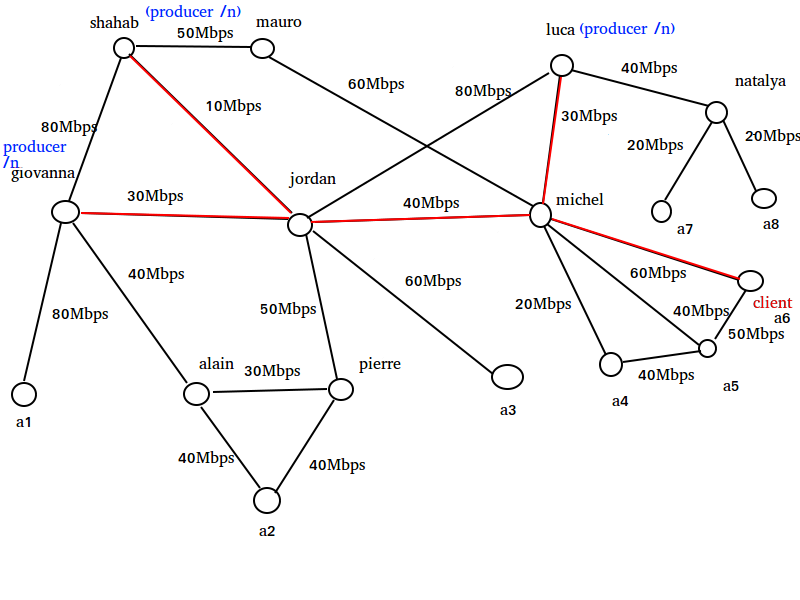
\includegraphics[scale = 0.5]{Figures/TreeOnProducer_big.png}

\caption{TreeOnProducer Tree Medium} \label{TreeOnProducer_big} 


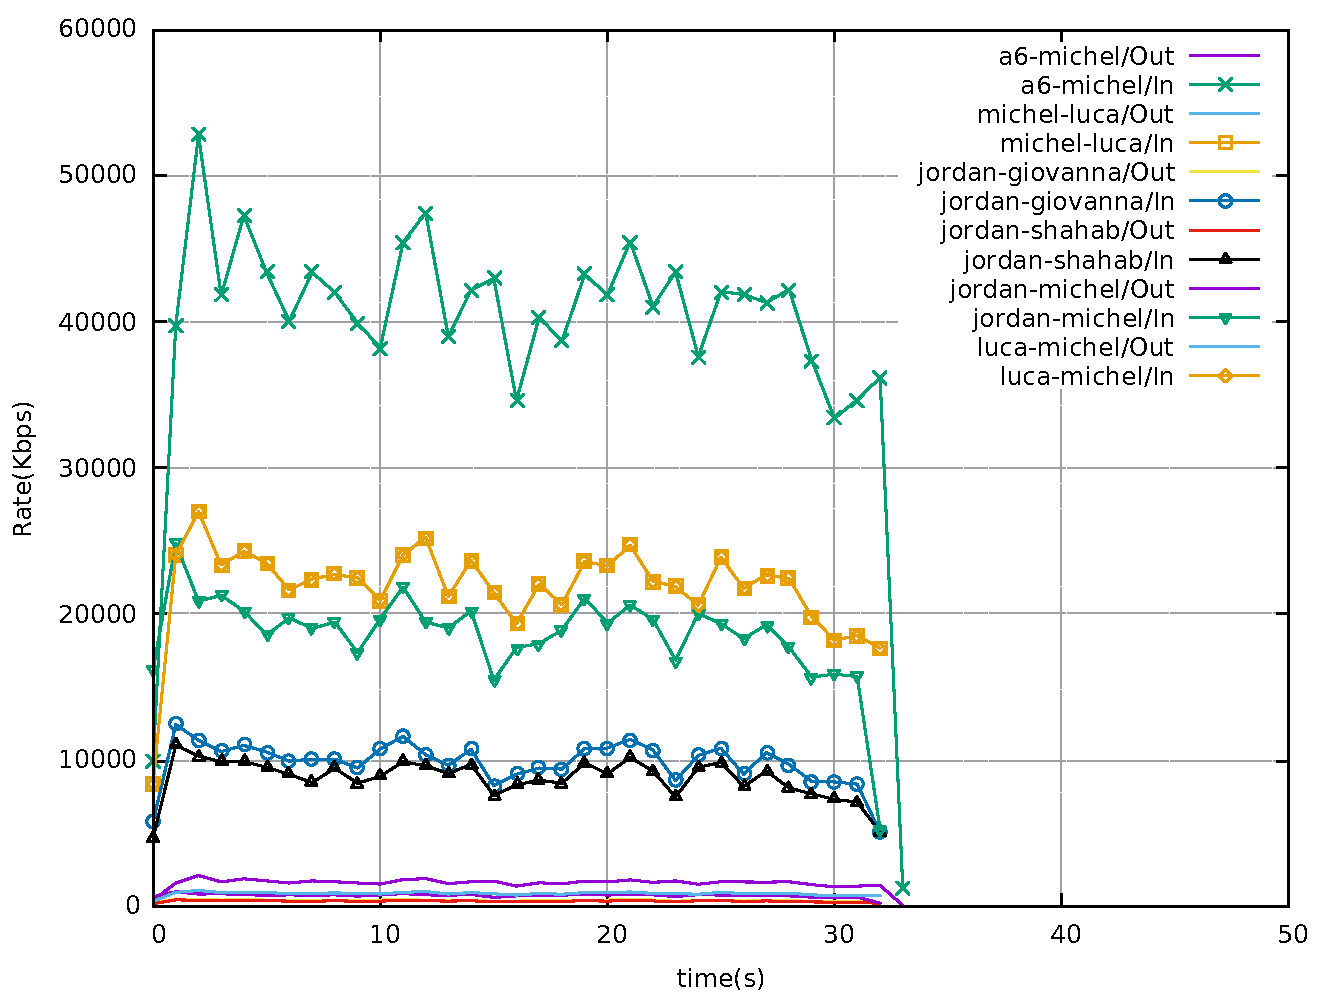
\includegraphics[scale = 0.5]{Figures/TreeOnProducer_big.pdf}

\caption{TreeOnProducer (Rate vs Time) Large} \label{treeonproducer_big} 


\end{center}

\end{figure}


\subsection{MinCostMultipath}
Figure \ref{MinCostMultiPath} shows how the \textit{MinCostMultiPath} tree is chosen to deliver content to all clients which are connected to access points.
 
Notably this strategy can be used when you want to do a \textit{Equal Cost Multi Path} (ECMP) routing in which your minimized paths have equal cost to destination so we should use load-balance or multipath forwarding strategy to allow traffic to pass along the network. 

Figure \ref{Load} shows well a simple case usage of this strategy using \textit{load balancing} strategy to use multipath routing.

There is a very important issue in this case of strategy, and the important concept is that when the routing strategies has decided or multi faces for each node the forwarder strategy can not be more best-route! Actually in this case engine of forwarder should allow the kernel to pass packets through different faces. Kernel lets operates like a switch to forward the packets into th network.

By this way we see clearly that designing a routing strategy also depends on forwarding strategies. 

In NFD, there is different forwarding strategies \textit{best-route} which uses the best route in terms of cost link function. \textit{multicast} which send the packets in multicast way, \textit{broadcast} which pipeline all packets toward all, faces in PIT table. These namespaces has been implemented and used in our studied works and experiments.

\begin{figure}[H]

\begin{center}

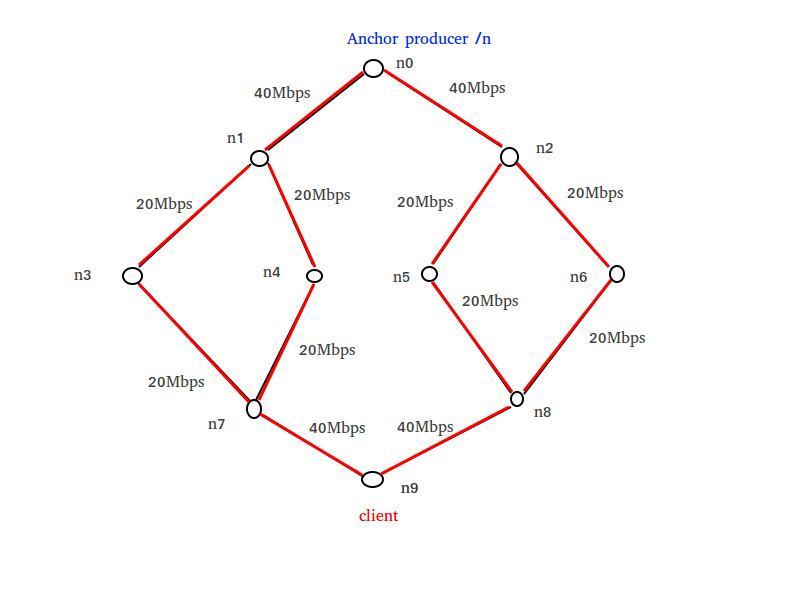
\includegraphics[scale = 0.5]{Figures/Load.png}

\caption{Multipath load balancing strategy Graph} \label{Load} 


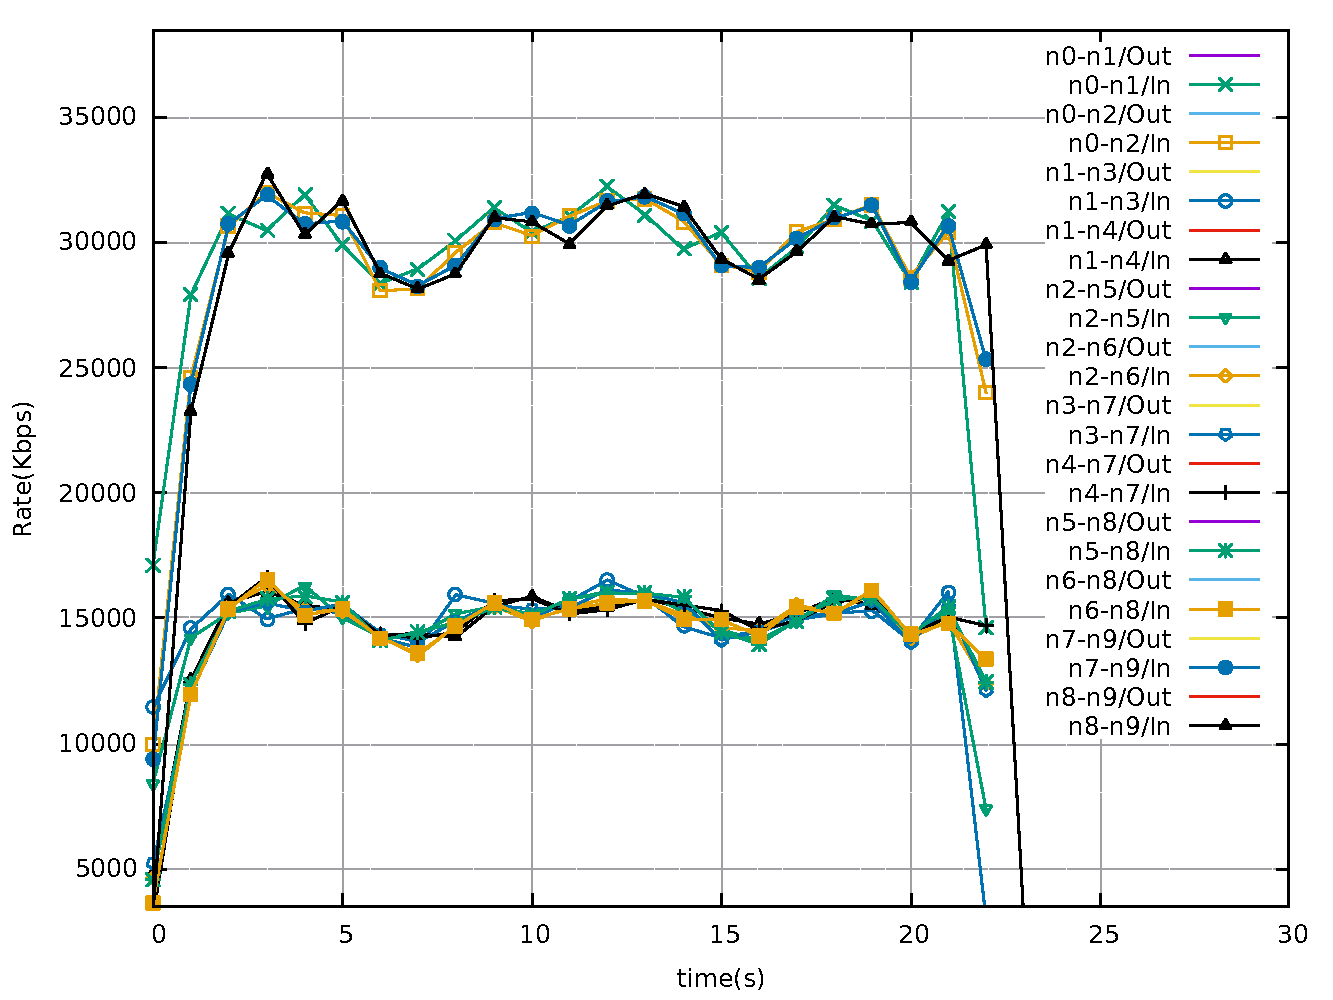
\includegraphics[scale = 0.4]{Figures/load.pdf}

\caption{Multipath load balancing strategy (Rate vs Time) } \label{load} 


\end{center}

\end{figure}




The algorithm of this strategy is written by the idea of searching minimum multipath from producer to client.

\begin{figure}[H]

\begin{center}

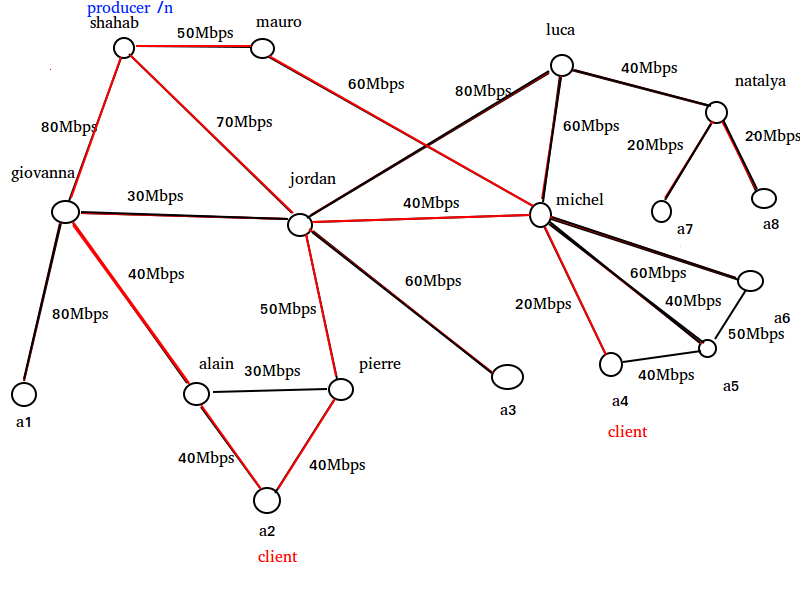
\includegraphics[scale = 0.4]{Figures/MinCostMultipath_big.png}

\caption{MinCostMultiPath Tree Large} \label{MinCostMultiPath} 


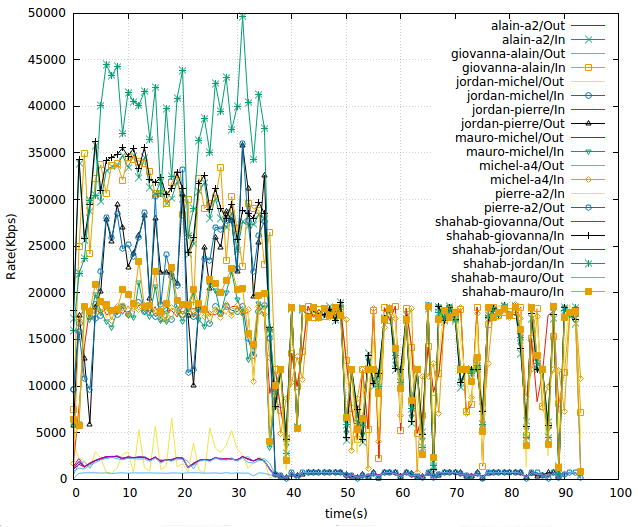
\includegraphics[scale = 0.4]{Figures/mincostmultipath_big.png}

\caption{MinCostMultiPath (Rate vs Time) Large} \label{mincostmultipath} 


\end{center}

\end{figure}


\textbf{\Large{Multi Consumers and Producers}}. Figure \ref{Multi-Repo-Client} as you can see we can have $n$ producers and $m$ consumers want to download at the same time. This strategy chooses the shortest paths between clients and consumers using to give routes update. Actually for each consumer, algorithm looks which producer is closer using \textit{shortest path} then set routes properly. This strategy can be very useful in ICN networks because of its architecture. 

Routing is the core issues of any network even Network of streets and broadways! It's the idea of Routing in general is to have knowledge about network and its proper graph then have a table at each router to calculate best routes for each packet. This table can be static or dynamic, normally in practice routers are dynamic in function of network needs. 

One beautiful idea which is very \textit{à la mode} in research and development in these days because of its advantages is to have a \textbf{S}oftware \textbf{D}efine \textbf{N}etwork. The SDN can be a central controller who allows users to modify the network in terms of capacities, network topology, routing, and whatever you can think about the network which can be changes dynamically.

You can also imagine a scenario to occur, you can have algorithms inside algorithms to run full automate evidences. This strategy can be very useful in these scenarios because of NDN architecture.

By running this strategy on Lurch, it can understand whenever you want to do a ECMP or Multi repository client. It's important because network when you have your controller (Lurch) who understands the scenario in which you want to apply your strategies. 

  


\begin{figure}[H]

\begin{center}


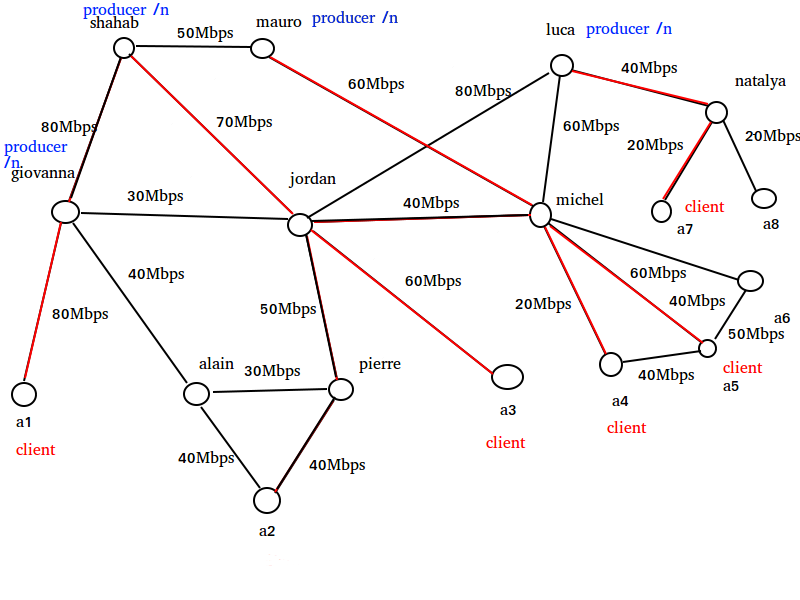
\includegraphics[scale = 0.5]{Figures/Multi-Repo-Client.png}

\caption{Multi Consumers and Producers Large} \label{Multi-Repo-Client} 


\end{center}

\end{figure}




\begin{figure}[H]

\begin{center}


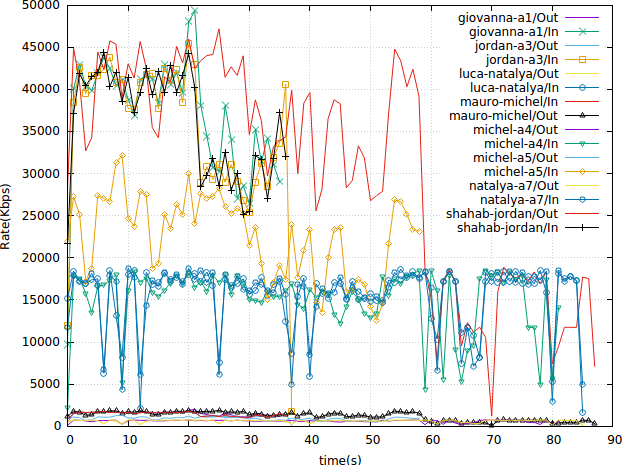
\includegraphics[scale = 0.4]{Figures/multi-repo-client.png}

\caption{Multi Consumers and Producers (Rate vs Time) Large} \label{multi-repo-client} 


\end{center}

\end{figure}

Now let's consider an interesting point of this strategy in Mobility of ICN. Figure \ref{Step1} shows the first step of a mobility scenario in which producer is attached to n18. In this case producer can be a Robot carrying a webcam to capture a film from environment send it to network as the content producer. The clients are mobile stations and are attached to base stations as well.   


\begin{figure}[H]

\begin{center}


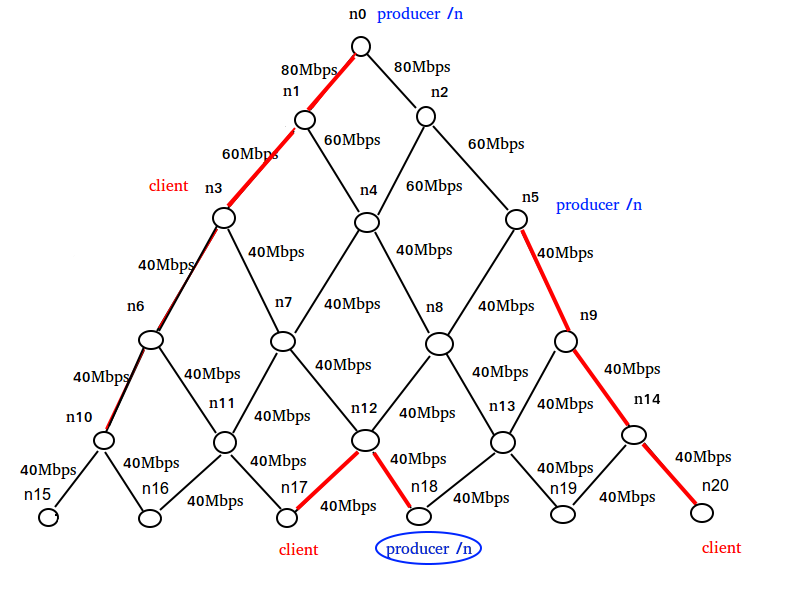
\includegraphics[scale = 0.4]{Figures/Step1.png}

\caption{Producer Mobility step 1 \& Routing update} \label{Step1} 


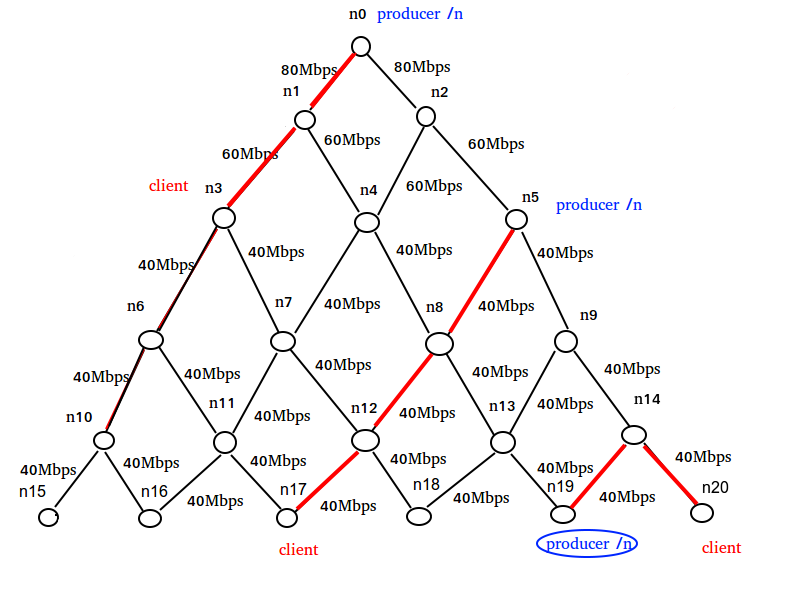
\includegraphics[scale = 0.4]{Figures/Step2.png}

\caption{Producer Mobility step 2 \& Routing update} \label{Step2} 

\end{center}

\end{figure}






\begin{figure}[H]

\begin{center}

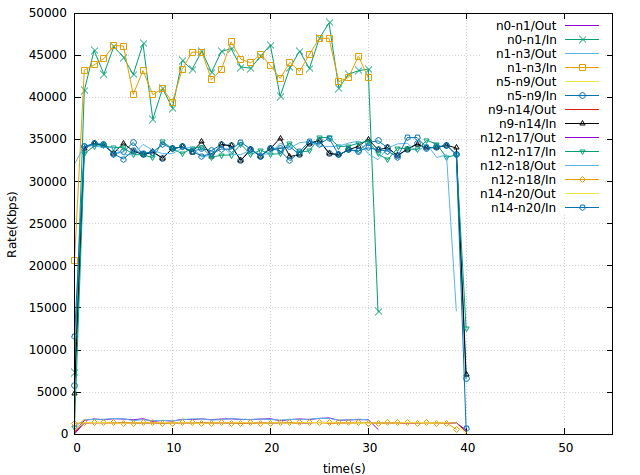
\includegraphics[scale = 0.4]{Figures/step1.png}

\caption{Producer Mobility step 1 (Rate vs Time) Large} \label{step1} 


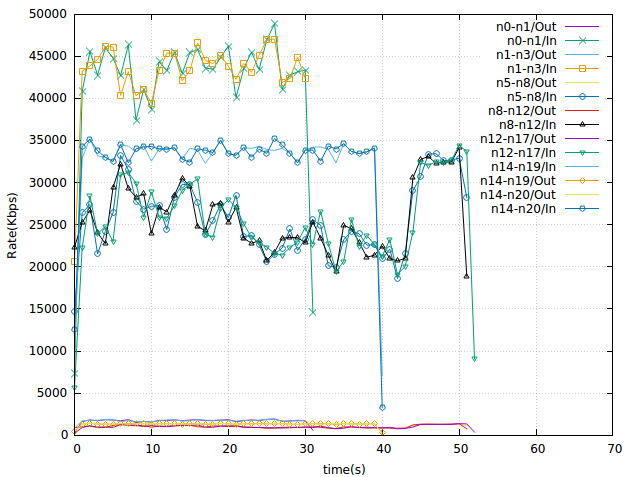
\includegraphics[scale = 0.4]{Figures/step2.png}

\caption{Producer Mobility step 2 (Rate vs Time) Large} \label{step2} 


\end{center}

\end{figure}



Now let's consider a case which i call it \textit{Dense} network because the number of clients and repositories are more than rests.

Figure \ref{Dense} shows well automatic routing best shortest path for each consumer to achieve to producers using this strategy.

Figure \ref{dense} shows also the stairs of rates falling down in the network because of waterfall sense of Network. Basically more you go deeper to network the capacity rate will be increased which is real assumption in networks because (backbone / backhaul / Mobile edge, ...)
\begin{figure}[H]

\begin{center}


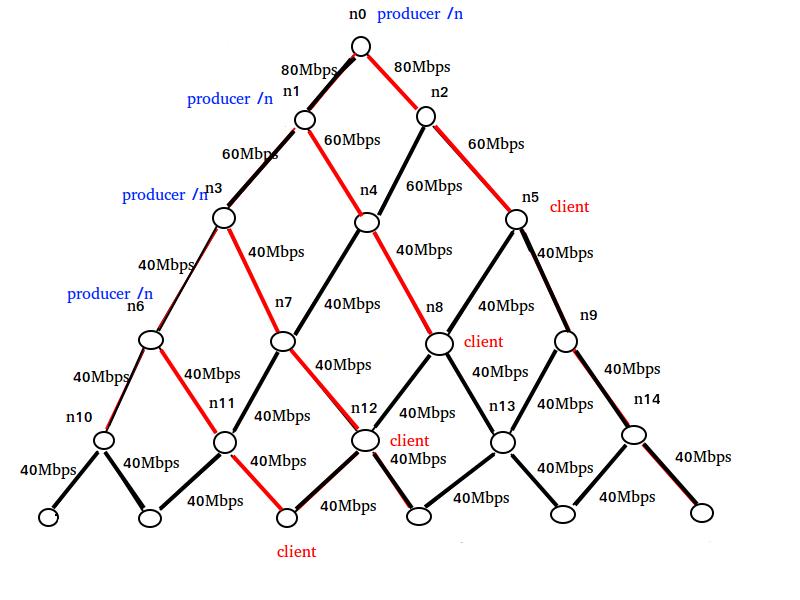
\includegraphics[scale = 0.4]{Figures/dense.png}

\caption{Dense Network} \label{Dense} 

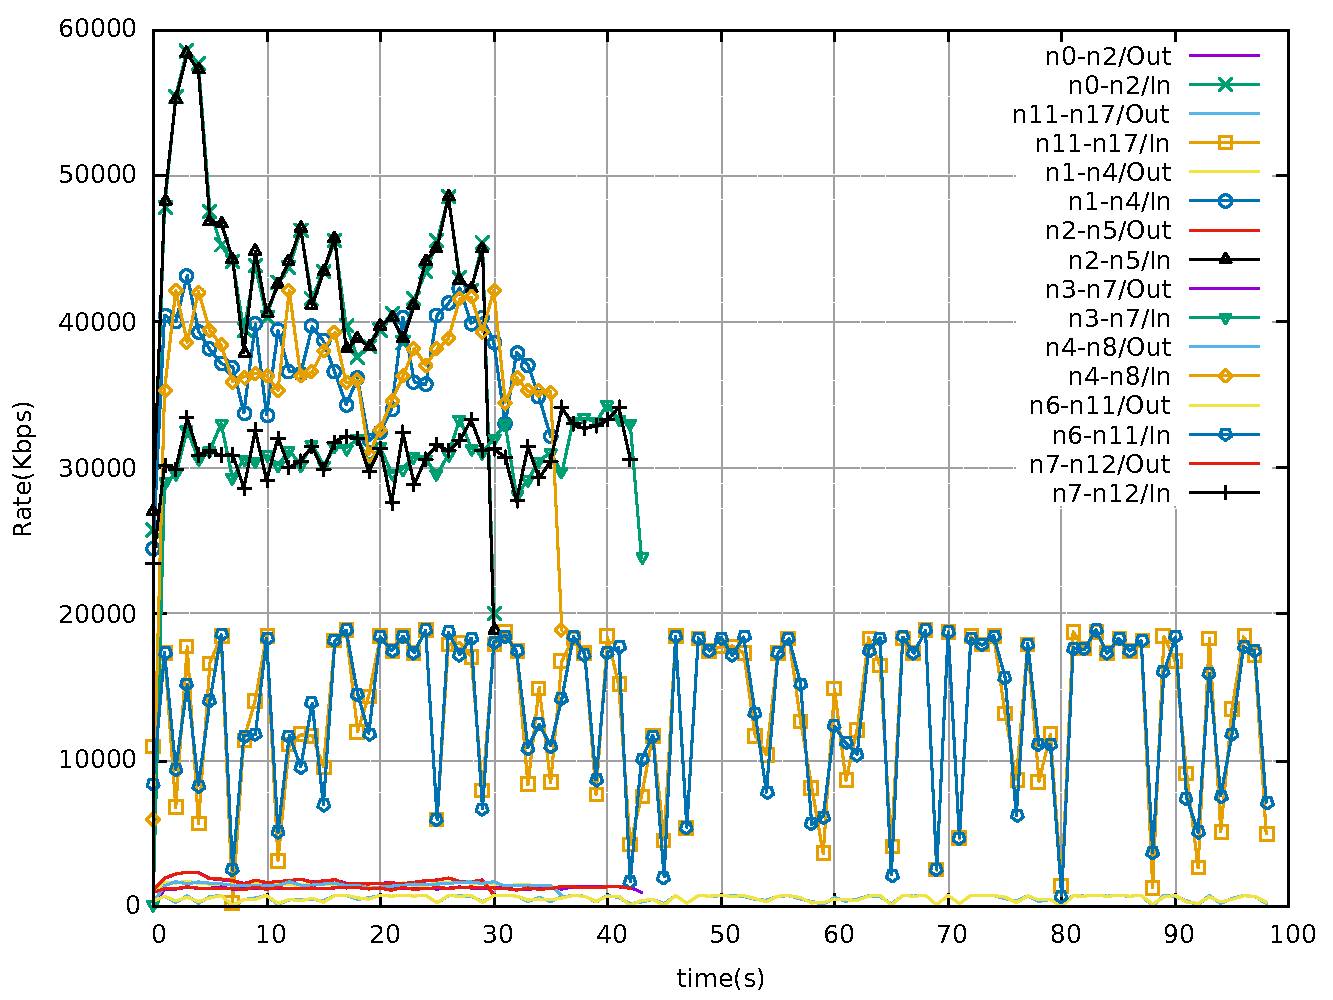
\includegraphics[scale = 0.4]{Figures/dense.pdf}

\caption{Dense Network (Rate vs Time) Large} \label{dense} 


\end{center}

\end{figure}












\subsection{MaxFlow}
Figure \ref{MaxFlow_big} shows the paths chosen by strategy to maximize the throughput. This strategy works with capacity of each link and according to these values it returns the paths which can maximum the throughput toward clients.

Figure \ref{maxflow_big} shows how the rates are changing during time with this strategy. As you can see data packets have maximum value to achieve the output.  

The mobile stations are connected to $a2,a3$ Access Points, they can download their contents through taps interfaces.

The algorithm of this strategy is written by finding the paths which maximize throughput with preventing out of range extra loops.

This algorithm finds the paths which is able to pass the packets from consumer to clients which maximizes the  total throughput. This allows you to use maximum capability of packets and whole of network usage which is quiet good for a high rate communication.

\begin{figure}[H]

\begin{center}

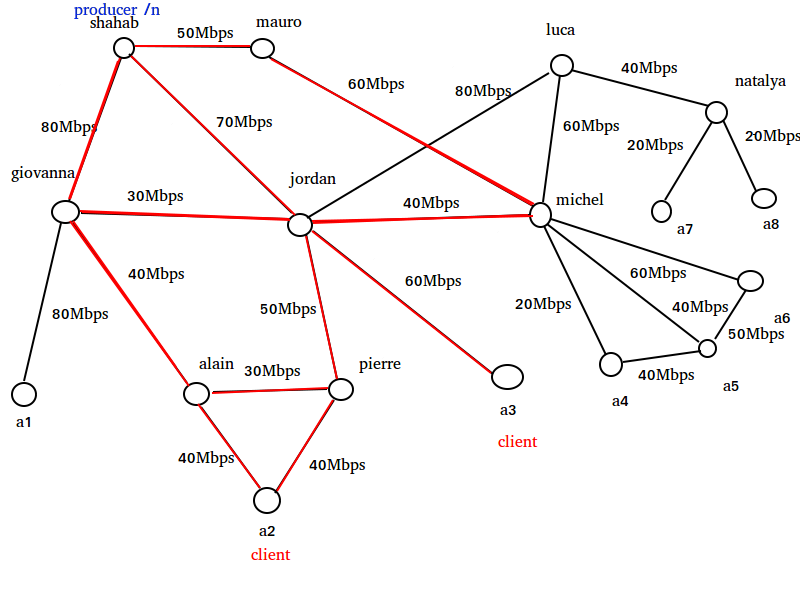
\includegraphics[scale = 0.4]{Figures/MaxFlow_big.png}

\caption{MaxFlow Tree Large} \label{MaxFlow_big} 


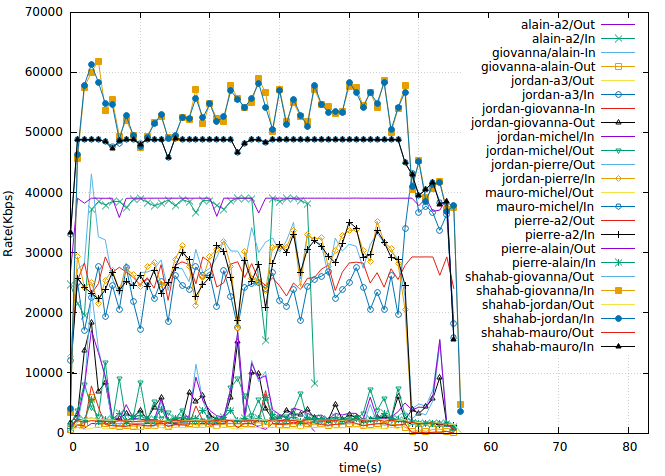
\includegraphics[scale = 0.4]{Figures/maxflow_big.png}

\caption{MaxFlow (Rate vs Time) Large} \label{maxflow_big} 


\end{center}

\end{figure}



